\chapter{Implications and Open Topics}
\label{chapter:implications}


\chapterprecishere{Freedom only remains healthy if we think about the implications of what we do on a day-to-day basis.\par\raggedleft--- \textup{Rebecca MacKinnon}}
\chapterhung

In this chapter we evaluate the risks and implications on systems that use \elektra{}, answering \rqref{implication}:
\rqImplication*

Our main concerns are the topics effected most by \elektra{}.
We look into impact on users.
We rely on case studies, experience, and ideas---fully conducted experiments and benchmarks follow in the next chapter.

In \secref{administer}, we look into the administration of the key database.
We present implications and risks of \elektra{Spec} for system administrators.

In \secref{tooling}, we discuss the impact \elektra{} has on tooling and show user interfaces.


In \secref{development}, we consider implications on development.
In a case study, we found that development time is reduced and quality improved.
We look into maintenance of applications using \elektra{}.


Finally, in \secref{security}, we reflect on the security, safety, and quality of \elektra{}.
We present some metrics of \elektra{}'s source code and then discuss implications concerning security and misconfiguration.


















\section{Administration}
\label{sec:administer}

One of the main goals of \elektra{} was to make administration of configuration settings easier in order to avoid misconfiguration.
Here we answer \rqref{implication-administration}:
\rqImplicationAdministration*


\subsection{Sharing of Configuration Settings}

As discussed so far, context awareness across applications implies sharing of configuration settings between applications.
Sharing is not always a good idea and imposes risks:
Sharing creates dependences between different communities.
Because communities can independently change the semantics of configuration values, sharing introduces co-evolution, which can lead to breakage.

A countermeasure in place is that we provide transformation of configuration values.
Using the transformation, we decouple applications from the exact configuration value other applications have.
But whenever an application changes its configuration settings, we need to update the transformation logic.
Supporting different versions of configuration specifications can lead to a complex transformation logic.

We suggest another solution:
Instead of directly sharing configuration settings between applications, we propose to use agreed shared places.
From these agreed shared places, applications transform their configuration settings, as hinted in \exref{shortcut}.
There does not need to be a single central organization for such reusable configuration settings.
Instead projects like \url{EditorConfig.org} specify configuration settings to solve specific configuration integration problems.
This way, the risk of changes in the configuration specification is reduced and configuration specifications have clear ownerships.

Because of the configuration specification, ^/etc^ can be left completely empty by default.
A system administrator only needs to add settings to the agreed shared places.
Applications would calculate their default values from these agreed shared places.
Using this procedure, \elektra{} fulfills Requirement~\reqref{integration}:
\reqIntegration*

It is future work to evaluate the efficiency of mitigation strategies to co-evolution.



\subsection{Documentation}

\empha[documentation]{Documentation} is a valuable artifact.
To enable social coding and to understand the intention of the specifications, we need further properties that document the specification, contributing to the requirement:
\reqDocumentation*

Even though some tools infer validation specifications~\cite{nadi2014mining,kiciman2004discovering,xu2013blame}, most parts of the configuration specification must be populated and maintained manually~\cite{mens2005evolution,chow2008survey}.
This applies in particular to documentation.
While the type and defaults are already part of the configuration specification in \elektra{}, other documentation needs additional properties.
We explain some further properties improving documentation with the aid of an example extending on \exref{introduction-openldap-crash}:

\begin{code}
[slapd/threads/listener]
  check/range:=1,2,4,8,16
  default:=1
  description:=adjust to use more threads
  rationale:=needed for many-core systems
  requirement:=1234
  accessibility:=platform engineers
\end{code}

The first line contains the most important information:
It specifies the existence of a configuration setting and its name.
The second line tells the system administrator which configuration values are permitted to be present.
Line~3 is already less important for system administrators.
It is more reliable to introspect configuration values because this reduces the danger of oversight.

The property \property{description} in line~4 contains only as much information as necessary and focuses on behavioral descriptions.
It does not repeat other parts of the specifications.
In particular, it does not repeat other specifications, such as default values.
Hand-written documentation that duplicates information from the source code is known to be error-prone~\cite{rubio2010expect}.
Instead the description should describe the configuration setting from the application's perspective.

The property \property{rationale} is an explanation of why the configuration setting is needed and why it is specified as it is.
Following the concept of documenting architectural decisions~\cite{zdun2007patterns}, only configuration settings are added if a clear demand for them exists.
Possible reasons for adding a configuration setting are:
%<*reasons-adding>
\begin{enumerate}
\item a requirement,
\item an architectural decision,
\item a technical need, and
\item an ad hoc decision.
\end{enumerate}
%</reasons-adding>


For the first three reasons the configuration settings need revalidation on influencing events, for example, on changes in requirements, decisions and technology.
Traceability links~\cite{ramesh2001toward} are useful to detect influencing events.
Ad hoc decisions need to be revalidated periodically.
If customers never change configuration settings---because the default value is already the optimal solution---the configuration setting and specification shall be removed.%
{\parfillskip=0pt plus .8\textwidth \emergencystretch=.5\textwidth \par}

For most stakeholders only some configuration settings are relevant.
The property \property{accessibility} defines who is responsible for a particular key in the configuration specification.
Tools filtering for this property present only relevant configuration settings to the respective stakeholders.
For example, in a graphical user interface the visibility of a configuration setting is directly derived from accessibility levels.

The risks of these suggestions are:
\begin{itemize}
\item
That important documentation is missing because no property is obligatory.
\item
That unnecessary documentation is added for the sake of having a complete set of documentation properties.
\item
Enforced properties might have more severe effects than wrong documentation.
For example, the property \property{accessibility} can cause problems:
If the property is assigned too strict, some stakeholders will not find the configuration setting they are looking for.
\end{itemize}
Thus configuration specifications need to be subject of maintenance by the application's developer.
Bugs in the configuration specification need to be handled like other bugs.


\subsection{Validation}

In \elektra{}, configuration specifications are not hard coded in applications and can be extended by system administrators.
Because ^kdb.set^ always enforces validation, system administrators that only use tools based on \elektra{Lib}, fulfill the requirement:
\reqValidate*

Without configuration specifications, \elektra{} works completely without any configuration validation.
Every configuration value is either a string or binary data with any content.
This behavior addresses the need to have a low barrier for \elektra{}'s adoption.
On the downside, the behavior adds the risk that system administrators forget adding configuration specifications.

Introducing the \intro[two-phase type checking]{two-phase type checking} has important consequences for the daily work.
It separates checks intended to be extended by developers and system administrators.
The first phase (structure check) is usually tightly interwoven with the application's configuration settings.
Writing such plugins is a challenging development effort and thus usually is not done by system administrators.

System administrators usually know pattern-matching languages such as globs and regular expressions well.
Thus they can employ the plugin \plugin{validation} to strengthen checks for their purposes:

\begin{code}[morekeywords={match}]
[slapd/logfile]
  check/validation:=/var/log/.*\.log
  check/validation/match:=word
  check/validation/message:=Policy violation: must be /var/log
\end{code}

Other plugins check if configuration settings are consistent with the context.
Such plugins can check the validity of network addresses and the existence of paths in a file system.
For example, to check if the configuration setting points to a existent file, system administrators use:

\begin{code}[morekeywords={path}]
[slapd/logfile]
  check/path:=file
\end{code}

Because of the vast amount of possibilities for checking values to be consistent with context, it is essential that system administrators are able to invent new kinds of consistency checks.
In our design, system administrators combine their own checks with the application developer's predefined structure checks.
It remains future work to evaluate up to what extent system administrators successfully combine different validation techniques.


\subsection{Error Messages}

Currently, system administrators are often confronted with applications behaving wrongly and not starting up.
Employing \elektra{}, they would instead encounter error messages from plugins rejecting their misconfigurations.
To make their work easier, it is essential that the plugins give good error messages.
Having human-friendly error messages is challenging~\cite{lee2011personifying,zhang2014configuration,loncaric2016practical}.
Using \elektra{} we have, however, a distinctive advantage:
During execution of ^kdb.set^ plugins know which keys were changed.


We use information about last-changed keys (a modification bit in metadata $\mu$) to improve error messages by a simple heuristic:
If several keys are potential causers of an error, we prefer those in the error message that were changed by the user.
\begin{example}
Given the specification:

\begin{code}[morekeywords={assign,math}]
[a]
  check/type:=long
[b]
  check/type:=long
[c]
  check/range:=0-10
  assign/math:=../a+../b
\end{code}

If we change ^b^ to 10 and ^a^ remains unchanged with 5, we have in the following in-memory configuration settings to be processed by ^kdb.set^:

\begin{code}[language=CfgElektra]
a=5  ; unmodified
b=10 ; modification bit in metadata is only set here
c=15 ; unmodified by user but changed later by assign/math
\end{code}

\elektra{} is capable to inform the user that ^b^ was set to an invalid value, even though the validation failed at ^c^:

\begin{verbatim}
  Sorry, I was unable to change the configuration settings!
  Description: I tried to set a value outside the range!
  Reason: I tried to modify b to be 10 but this caused c to be
          outside of the allowed range (0-10).
  Module: range
  At: sourcefile.c:1234
  Mountpoint: /test
  Configfile: /etc/testfile.conf
\end{verbatim}
\end{example}

For the error message, we are only interested in keys changed by the user.
This way we can pinpoint to a likely source of the error.
Unfortunately, plugins need to implement this feature, and the heuristic can fail.

The error message is personalized and starts with ``Sorry'' and ``I''.
This eye catcher is relevant to improve novice\footnote{
And as we know, also expert developers and system administrators start as novice when using a new tool.} programmers' learning.
\citet{lee2011personifying} found in a study with a programming game that participants receiving personalized feedback \enquote{completed significantly more levels in a similar amount of time}.
Future work is needed to evaluate the impact of such error messages on the daily work of system administrators.


\subsection{Context-aware Lookup}

If possible, we prefer tools to automatically avoid problems and not only to check for them.
Here we consider implications of \elektra{Spec} as a high-level programming language with its context-aware lookup features.

Links already allow us to implement simple logics.
We easily add new rules where configuration settings shall be searched for.
\begin{example}

\label{ex:override-argument}
Let us determine if one of the arguments is set to true, i.\,e., the string~^1^:

\begin{code}[morekeywords={override}]
[sw/org/abc/has_true_arg]
  type:=boolean
  default:=0
  override/#0:=/sw/org/abc/arg0
  override/#1:=/sw/org/abc/arg1
\end{code}

Using ^override^ we specify a list of arguments that ensure that the key ^/sw/org/abc/^ ^has_true_arg^ yields true if one of the ^arg^$N$ is true.
\end{example}

\empha[cascading lookup]{Cascading lookup} requires all namespaces to be inquired exhaustively.
\citet{evard1997analysis} proposes to use cascading lookup but only at configuration file level.
\elektra{} extends these ideas to individual keys.
Administrators employ cascading lookups of applications to have different configuration settings:
\begin{itemize}
 \item to try out new configuration settings via command-line options and environment variables (^proc^ namespace),
 \item if the application is started from different directories (^dir^ namespace), and
 \item for different users (^user^ namespace).
\end{itemize}

System administrators facilitate the cascading lookup to know the configuration settings an application currently uses---without any manual calculations or guesswork.
We fulfill Requirement~\reqref{introspection}:
\reqIntrospection*

A \empha{layer-based lookup} includes even more possibilities to consider context.
We gain flexibility but also make the introspection more difficult.
With dynamic scoping, the configuration setting can even change for different parts of the same application.
We are still able to introspect each of the possibilities but which of these is used depends on the layers within the threads and dynamic scopes.

Except for the layer-based lookup, we gain a futz-free system to introspect configuration values.
It remains as future work to evaluate the layer-based lookup from the system administrator's viewpoint.



\subsection{Discussion}

Here we conclude the answer to \rqref{implication-administration}:
\rqImplicationAdministration*


\citet{evard1997analysis} said: \enquote{A good abstraction model changes the way in which one thinks.}
Allowing programming of configuration access widens the spectrum of how system administrators control their systems.
Instead of seeing configuration access as a black box, with \elektra{Spec} they get possibilities to introspect and even program configuration access.
System administrators finally get ways to:
\begin{itemize}
\item share configuration settings,
\item document configuration settings at specified places,
\item make configuration validations stricter with more specific error messages, and
\item derive configuration settings from context and requirements.
\end{itemize}


\elektra{Spec} blurs the line of responsibility between developers and system administrators, which involves risks:
\begin{itemize}
\item
System administrators need to learn more concepts and need more programming background.
Some of \elektra{}'s concepts are difficult to grasp, for example, the context-aware lookup.
\item
System administrators can loosen or change validation specifications in wrong ways.
Such actions not only open doors for misconfiguration but the tools even give wrong statements about valid configuration settings.
\item
System administrators can use wrong plugins, or can implement plugins wrongly.
\item
System administrators might get even less help in case of misconfigurations because developers may suspect system administrators to have failed in one of the points above.
\item
Layer-based lookups in frontends are too flexible to fully cover Requirement~\reqref{introspection}.
\end{itemize}





















































\section{Tooling}
\label{sec:tooling}

A consequence of \elektra{Lib} is that configuration management tooling does not need to be bothered with mechanics how to manipulate specific configuration files.
With respect to the parts that \elektra{Spec} dictates, the tooling has consistent behavior.
In this section we discuss the implications on tooling.


\subsection{Configuration Management}

While many approaches for \empha{configuration management}~\cite{cons2002pan,huang2015confvalley} exist, they lack good support for consistent configuration file manipulation and introspection.
In the current situation, the user of the configuration management tool is either severely restricted in which configuration settings can be changed, or needs to have a working knowledge about the syntax of involved configuration files.
Configuration management tools have limited possibilities to detect syntactically wrong and non-validating configuration files, especially if the errors result from context.

\elektra{} is a good fit for these problems. Using \elektra{}
\begin{enumerate}
\item
the mechanisms of how to manipulate configuration files is reduced to key-value manipulations,
\item
with correctly-working storage plugins it is impossible to create syntactically incorrect configuration files (assuming every key name and every configuration value is representable in the respective syntax),
\item
configuration settings are always validated before they are serialized to configuration files, and
\item
via introspection the current state of the system can be queried.
\end{enumerate}

The disadvantage is that \elektra{} needs to be installed and all configuration files need to be mounted.
Furthermore, some concepts such as cascading lookup is not needed for configuration management and introduces complexity.



\subsection{Text Editor}


Because \elektra{} usually parses and serializes configuration files from the hard disk, system administrators can still access these configuration files with a text editor.
Directly manipulating configuration files, however, does not respect validation, syntax, and notification constraints \elektra{} otherwise would enforce.
Hence, we do not recommend bypassing \elektra{}.
One solution is to consequently rely on ^open^ interception, i.\,e., configuration files are not present in the file system but always passed through \elektra{}.
In general, however, such a solution is too heavyweight.

As an alternative, \elektra{} provides a small wrapper around text editors.
The wrapper's functionality is that it exports the configuration settings to a temporary file and spawns the users' favorite editor with this temporary file.
After the editor has terminated successfully, the wrapper tries to import the configuration file.
During the import \elektra{} enforces correct syntax and validation.
This way, we provide a work flow and user experience almost identical to directly editing configuration files.


\subsection{Command-line Interface}
\label{sec:implication-command-line-interface}

We created a command-line tool ^kdb^ that maps all features of the configuration access API to the command-line.
It is straightforward to transform the declarative syntax we used in this book to imperative ^kdb^ commands.
\begin{example}
Suppose we want to have the configuration settings:

\begin{code}[language=CfgElektra]
a=5
b=10
c=15
\end{code}

We apply these configuration settings using:

\begin{code}[language=bash]
kdb set /a 5
kdb set /b 10
kdb set /c 15
\end{code}

And we list them with \lstinline[language=bash,morekeywords={ls}]^kdb ls /^.
\end{example}

\vspace{1em} % example clash

\begin{example}
For specifications such as:

\begin{code}
[slapd/threads/listener]
  check/range:=1,2,4,8,16
  default:=1
\end{code}

We use:

\begin{code}[language=bash,morekeywords={setmeta}]
kdb setmeta /slapd/threads/listener check/range 1,2,4,8,16
kdb setmeta /slapd/threads/listener default 1
\end{code}

And we list them with \lstinline[language=bash,morekeywords={lsmeta}]^kdb lsmeta /slapd/threads/listener^.
\end{example}

Given a specification we explore which key names exist with tab completion (implemented for ^bash^, ^zsh^, and ^fish^, or use \lstinline[language=bash,morekeywords={complete}]^kdb complete^ otherwise).
For debugging purposes, the complete trace of which keys are considered by ^ksLookup^ are printed (^-v^ option of \lstinline[language=bash,morekeywords={get}]^kdb get^).
This functionality is implemented by using the hook ^lookupByExtension^.


\subsection{Graphical User Interface}

\figref{gui} shows a screenshot of the graphical user interface.
It was the second user interface after the command-line interface and provides undo functionality.

\begin{figure}[htp]
\centering
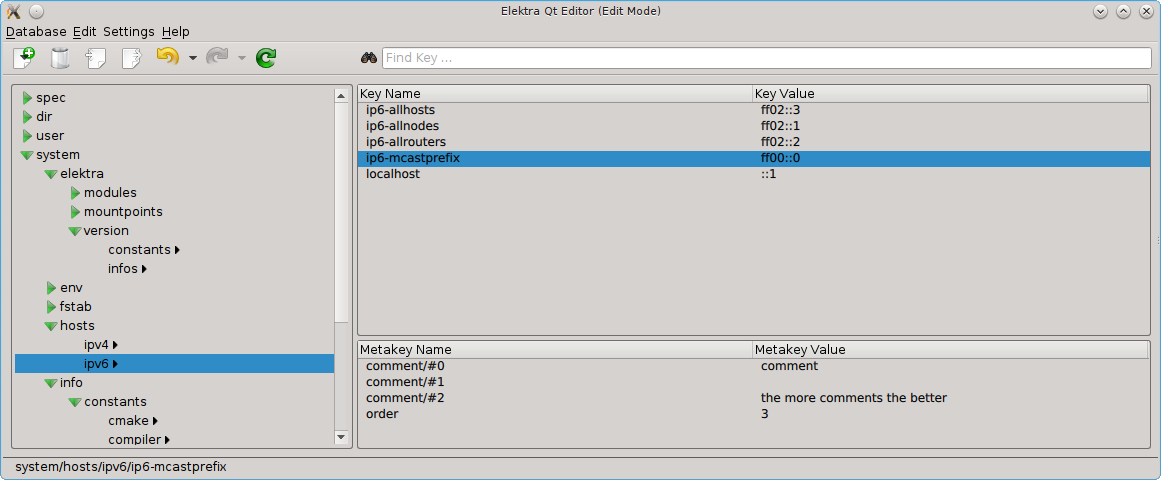
\includegraphics[width=\textwidth]{gui}
\caption{Graphical User Interface of \elektra{}.}
\label{fig:gui}
\end{figure}

\subsection{Web User Interface}


\begin{figure}[htp]
\centering
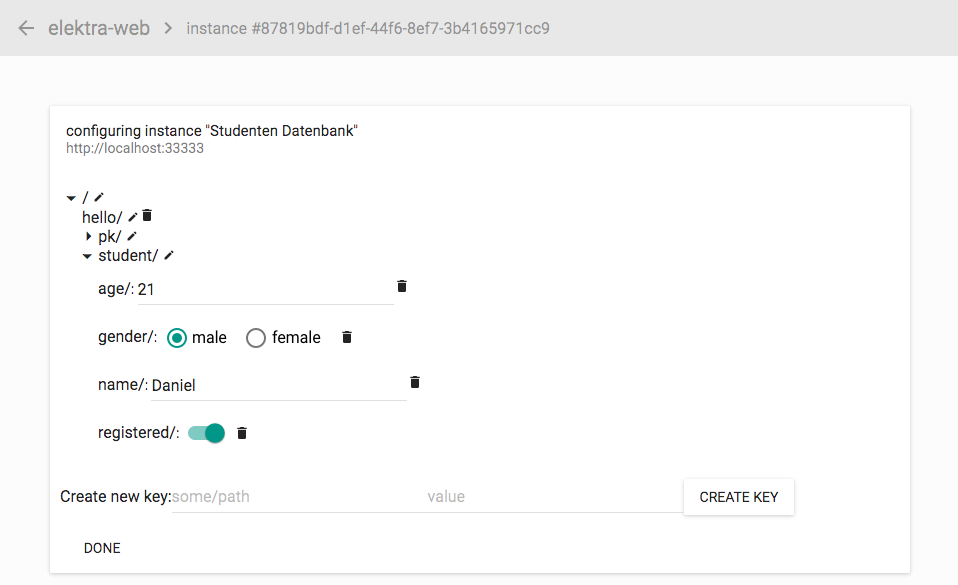
\includegraphics[width=\textwidth]{webui}
\caption{Web user interface of \elektra{}.}
\label{fig:webui}
\end{figure}

\figref{webui} shows a screenshot of the Web user interface.
During the still ongoing implementation of the Web user interface, we explore to what extent a user interface can avoid misconfiguration even earlier.
The idea is to avoid text fields but instead let the user choose between known-to-be-valid configuration settings inferred from \elektra{Spec}.
\begin{example}
Suppose the administrator wrote the specification:

\begin{code}
[hello/pk/student/registered]
  check/type:=boolean
\end{code}

Here the user interface provides a checkbox, making it impossible to enter anything except true or false.
\end{example}


\subsection{Converting Configuration Settings}

Another implication of the common data structure is that we can freely convert between any of two converted formats in \elektra{} as shown in \figref{convert}.
This is useful for importing and exporting configuration settings.
It can help for upgrades if the configuration file format changed.

\begin{figure}[htp]
\centering
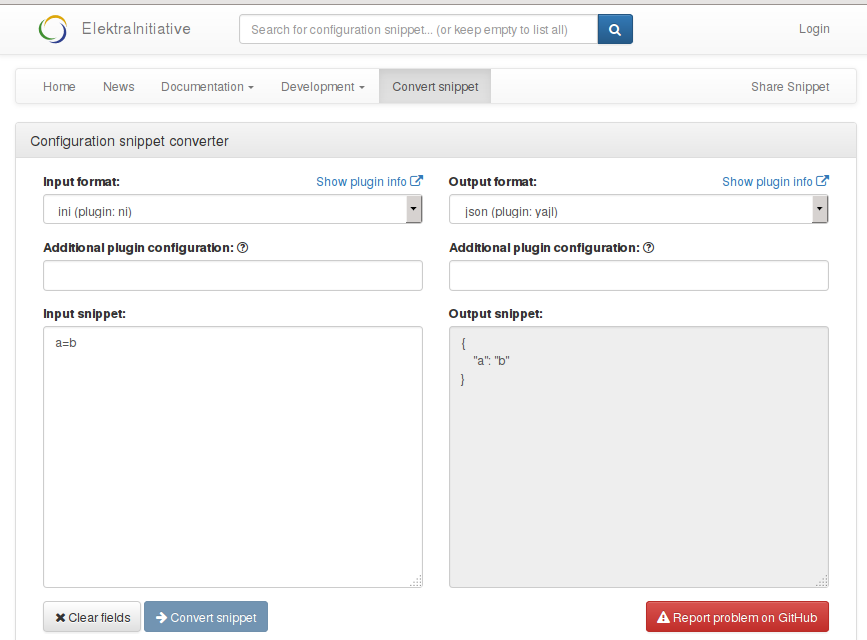
\includegraphics[width=0.8\textwidth]{convert}
\caption{Convert configuration settings with \elektra{}.}
\label{fig:convert}
\end{figure}

The conversion enables us to integrate configuration settings as source code.
We wrote the plugin \plugin{c} that outputs the configuration settings as C code.
Applications include and compile these files to have built-in configuration settings.


\subsection{Discussion}

\elektra{} has advantages for tooling:
\begin{itemize}
\item System administrators use configuration management tools easier with and more confidence:
Configuration files automatically use the correct syntax and invalid configuration settings get rejected.
\item User interfaces utilize information from \elektra{Spec}:
They show descriptions and even restrict input fields to improve usability.
\end{itemize}

Using \elektra{} involves risks:
\begin{itemize}
\item
If system administrators or applications forget to mount a configuration file, configuration settings are serialized to unwanted places.
\item
The user is dependent on plugin's decisions with respect to the formatting of configuration files.
Some plugins reformat to consistent but potentially unwanted style.
Other plugins aim at preservation of the original format, which is not ideal if configuration files are formatted in a chaotic style.
\item
System administrators might get careless when they edit configuration settings because they expect their errors to be caught.
\item
New tools may be refused by system administrators who are used to manipulate configuration files with their self-written tools.
Depending on the setup, bypassing \elektra{} by directly modifying configuration files is possible, but it is never recommended.
\end{itemize}








































\section{Development}
\label{sec:development}

In this section, we give experience reports with the lessons learned in software projects using \elektra{}.

\rqsubsection{implication-development-time}{Case Study: Development Time}

We investigate \rqref{implication-development-time}:
\rqImplicationDevelopmentTime*

\subsubsection{Method}

We developed an integrated camera system in a one-year engineering project.
The project combined development of software and hardware components.
The staff of the software team varied between three and five full-time software developers.
We wrote about 50,000 lines of C and C++ code.
We used Scrum~\cite{linda2000scrum} as agile development method~\cite{raab2015kps}.

The project aimed to engineer a platform for integrating different software applications.
The platform offered more than 200 configuration settings via \elektra{}.
The configuration settings affected both the platform and integrated applications~\cite{raab2015kps}.
Many of these configuration settings were relevant for system administrators.

Unfortunately, we did not do time measurements during the project.
Thus we redid the parts of the project relevant to configuration access in \elektra{}'s public repository~\cite{raab2015kps}.
We measured the time using stop watches or by calculating time from Git commits.
We argue that these time measurements are more realistic because of the background from a real-world project.
The shown source code is representative for what we did during the project.%
{\parfillskip=0pt plus .8\textwidth \emergencystretch=.5\textwidth \par}

\subsubsection{Case Study}

We got the basic setup for \elektra{} running within a day.
Hindering factors were that \elektra{} was not packaged everywhere and features for unusual requirements were missing.
The basic setup in the main program only consisted of the following lines~\cite{raab2015kps}:


\begin{code}[language=Cpp]
#include <camera.hpp>

int main ()
{
	using namespace kdb;
	KDB kdb;
	KeySet conf;
	Context c;
	Environment env (conf, c);
	std::cout << env.camera.name << "\n";
}
\end{code}


In the first line, we include the source code generated by \elektra{Gen}.
After creating a handle to the key database (line~6), we create a ^KeySet^ for configuration specifications, settings (line~7), and a ^Context^ (line~8)~\cite{raab2014program}.
Then we create an instance of the generated class ^Environment^ (line~9).
In line~10, we access a configuration setting.
Within minutes new developers started using these configuration settings~\cite{raab2015kps}.

To add a configuration setting is also simple.
We only needed 2 minutes to specify a new configuration setting and to use it in the application.
Because of this effort being so little, it is important to take care not to introduce unnecessary configuration settings~\cite{xu2015hey}.
Adding the ability to accept command-line options for the configuration setting was done within 6 minutes~\cite{raab2015kps}.

We heavily relied on the extensibility of \elektra{}, for example we invented new properties.
These properties are not described in this book because they are specific to requirements of that project.
Extending code generators and plugins to support the new properties had acceptable effort~\cite{raab2015kps}.


Within the same project we had difficulties to extend \elektra{} to further configuration file formats.
For example, to implement the NTP configuration file format, we estimated the implementation to need more than a week.
To improve on that situation, we evaluated different ways to implement new configuration file formats more quickly~\cite{raab2015kps}:


\begin{description}
\item[Existing Libraries:]
Integrating existing libraries requires low effort.
We must transform \elektra{}'s data structures to the data structures the existing library uses.
\begin{example}
The INI plugin \plugin{ni} (it implements the syntax of the examples in this book) had 158 lines of C code and was implemented within less than a day (10:41:54--16:22:01).
For parsing the properties of configuration specifications, in essence, the following source code suffices~\cite{raab2015kps}:

\begin{code}[language=Cpp]
Ni_node mcur = NULL;
while ((mcur = Ni_GetNextChild (current, mcur)) != NULL)
{
        keySetMeta (k, Ni_GetName (mcur, NULL),
                    Ni_GetValue (mcur, NULL));
}
\end{code}

The code parses a configuration specification in the syntax as used in this book.
\end{example}

For low-level, event-driven APIs the required effort is higher, even more than one week, for example, to parse JSON.
The main effort for the JSON plugin was to remember in which (sub)array and (sub)object the key currently is because the events do not give such hints.

A vast amount of configuration libraries suitable to be integrated in \elektra{} exist, and it is usually easily possible to avoid APIs causing extra effort.

\item[Using Grammars:]
Implementing storage plugins with grammars took us more time than using typical configuration libraries.
Grammars only mitigate the problem of how to parse but the serialization of the configuration files still needs to be done manually.
For parsing and serializing a TCL format we needed about three days (\formatdate{9}{8}{2010} 12:54:44--\formatdate{12}{8}{2010} 13:37:35).
The advantage of grammars is that changing the parsing code is as straightforward as changing the serializer code~\cite{raab2010thesis}.
\begin{example}
Using Boost.Spirit~\cite{raab2010thesis}, we needed the following parsing code:

\begin{code}[language=Cpp]
query = '{' >> *(pair) > '}';
pair = '{' >> key_name > '=' >> key_value >>
       *('{' >> metakey_name > '=' >> metakey_value > '}')
       > '}';
\end{code}
\end{example}


\item[Hand-written parsers:]
It is the most effort to implement a configuration file parser by hand.
For example, it took about \emph{one month} to implement a fully-fledged INI parser that preserves order and comments.
Adding many features needs considerable time---even for seemingly trivial parsers like CSV and hosts.
\end{description}

For extending \elektra{Gen} with new features we noticed a similar variety as in parsing.
The one extreme is that adding long option parsing support required less than one hour implementation time (10:53:30--11:33:04)~\cite{raab2015kps}.
The other extreme is implementing support for contextual values, which took many months and needed research to do it efficiently.
The entry barrier to support new properties turned out to be minimal.
Someone unfamiliar with \elektra{} wrote support for new properties within several days.

Code generation sometimes drastically reduces efforts.
In particular, many artifacts can be easily kept in sync by generating them from a single specification.
\elektra{Gen} currently allows us to generate code in C and C++ and documentation as man pages, Doxygen, and HTML.

Sometimes refactoring was needed when the hierarchy of the configuration settings was not adjusted to the features anymore.
In this situation, \elektra{Gen} was especially useful because we got immediate compilation feedback of all places that needed adjustment.
Developers easily forget where a configuration setting is used otherwise.


\subsubsection{Discussion}

We answer \rqref{implication-development-time}:
\rqImplicationDevelopmentTime*

\begin{finding}
We were able to use \elektra{} within a large real-world project successfully.
Many otherwise time-consuming tasks could be done within minutes or hours; in other cases \elektra{} did not help.
We did not have any requirement that could not be solved by extending \elektra{}.
Due to time reduction, \elektra{} increases risks that developers introduce too many configuration settings.
We are positive that the generation of artifacts related to configuration settings reduces co-evolution.
\end{finding}





\rqsubsection{implication-embedded}{Case Study: Embedded Web Server}
\label{sec:implication-embedded}

We implemented a Web server on an embedded hardware using the high-performance C++ Web development framework CppCMS~\cite{beilis2015cppcms}.
As target platform we chose a Raspberry Pi\textsuperscript{\textregistered} Model B because of its low prize and power consumption.
In this case study we answer \rqref{implication-embedded}:
\rqImplicationEmbedded*

\subsubsection{Case Study}

The configuration specification of all contextual values was only 83 lines long.
The specification contained basic settings needed to run a Web server, to work with hardware profiles, and to output tampering events.
Some of these contextual values are shown below.
From the configuration specification we generated 3500 lines of policy-based, nested C++ classes and command-line option parsing code~\cite{raab2014program,raab2015global}.

Contextual values are well suited to represent server side knowledge about an HTTP session.
We facilitated a specification that used the context placeholders ^%session%^ and ^%lang^\-^uage%^~\cite{raab2015global}:

\begin{code}
[sw/pi/%session%/language]
  type:=string
[sw/pi/%language%/hello]
  type:=string
\end{code}


In the first version of the Web server, we manually implemented the layers~\cite{raab2015global}.
In a second version, we instead used contextual values~\cite{raab2016persistent}.

\begin{example}
One of the first steps was to implement the HTTP request handler.
The object ^out^ is a stream to write the HTTP response~\cite{raab2015global}:


\begin{code}[language=Cpp]
tc.with<Session>(sessionid)([this]()
{
	out << "<html>\n"
		   "<body>\n";
	out << "<p>Language: " << language << "</p>";
	tc.with<Language>(language)([this](){
		out << "<p>" << hello << "</p>";
		//...
	});
	out << "</body>\n"
		   "</html>\n";
});
\end{code}

We use ^with^ to have the current session as thread-local context during the HTTP request handler.
\elektra{} changes all contextual values according to the session including the contextual value ^sessionid^.
Then we can activate the other layers, for example, ^language^.
When we output the contextual values, for example ^hello^, the output will match with the user's session and language settings~\cite{raab2015global}.
\end{example}


We want to avoid losing session information, for example, the selected language.
\elektra{} satisfies such persistence requirements by using the following two lines of source code~\cite{raab2015global}:


\begin{code}[language=Cpp]
{
  std::unique_lock<std::mutex> l = c.requireLock();
  kdb.set(ks);
} // automatic unlocked at end of scope
\end{code}

In the source code above, we require a lock using the ^Coordinator^ interface accessed with ^c^.
Afterwards, we use ^kdb.set^ to serialize the data structure ^KeySet ks^.
The key set ^ks^ contains all values for every context~\cite{raab2015global}.

In our study we were able to elegantly represent device-wide changes of contexts.
For example, our device was able to report tampering events using motion detection within an enclosure.
When opening the enclosure, the motion detection would trigger.
We used an infrared sensor HC-SR501 connected via the general-purpose input/output (GPIO).
On tampering events, we included the information on the delivered Web pages.
To implement this use case we specified a contextual value~\cite{raab2015global}:

\begin{code}
[sw/pi/tamper/%tamper%]
  default:=0
\end{code}

We used one thread to wait for tampering events via the system call ^select^.
If a tampering event occurs, ^select^ returns and we activate the layer ^Tamper^.
Eventually the contextual values in the other threads are updated.
We use the contextual value ^t^ (short for ^tamper^) to notify users via the delivered Web pages~\cite{raab2015global}:

\begin{multicols}{2}
\begin{code}[language=Cpp,xleftmargin=0ex,xrightmargin=0ex]
select (fd+1, 0, 0, &fds, 0);
context.activate<Tamper> ();


\end{code}

\columnbreak

\begin{code}[language=Cpp,xleftmargin=0ex,xrightmargin=0ex,breaklines=false,numbers=right]


t.context ().syncLayers ();
if (t) out << "tampered!";
\end{code}
\end{multicols}

Finally, \elektra{} enabled us to arbitrarily multiplex GPIO via layer activations.
We call the according layers \empha[hardware profile]{hardware profiles}.
A hardware profile is a layer that distinguishes between different hardware setups~\cite{raab2015global}.

\begin{example}
An excerpt of the configuration specification is~\cite{raab2015global}:

\begin{code}
[hw/pi/pi/%profile%/folder]
  type:=string
  check/path:=directory
  default:=~
[hw/pi/pi/%profile%/tamper]
  type:=string
  default:=tamper.txt
\end{code}

We used the specification with configuration settings such as~\cite{raab2015global}:

\begin{code}[language=CfgElektra]
hw/pi/pi/gpio/folder=/sys/class/gpio/
hw/pi/pi/gpio/tamper=gpio7
hw/pi/elitebook/gpio/folder=~/context/pi
hw/pi/elitebook/gpio/tamper=tamper.txt
\end{code}

With the hardware profiles, we were able to use ordinary files on our development laptop while using kernel interfaces on the embedded hardware.
Apart from simplifications during development, the hardware profiles enabled us to have different hardware setups with the same firmware image~\cite{raab2015global}.
\end{example}

As we see from the example, layer activation works without having the target hardware available:
We achieve a hardware abstraction~\cite{raab2015global}.

Contextual values easily emulate the functionality of profiles as described in \secref{frontend-history-context}.
Different from profiles, we are:
\begin{itemize}
\item not limited in the number of dimensions due to layers, and
\item not confronting every developer with the concept; without a need of layers activation, API users do not need to know about it.
\end{itemize}


\subsubsection{Discussion}

We answer \rqref{implication-embedded}:
\rqImplicationEmbedded*

\begin{finding}
We wrote a multi-threaded embedded Web server without having to take care about context and synchronization with the execution environment.
Instead all context specifications were short and located at a single place.
Hardware profiles implemented with contextual values enabled easier embedded development.

Manual implementation of layers was only needed in rare occasions, for example, to restrict contextual values to specific threads and processes.
\end{finding}




































\rqsubsection{implication-debugging-support}{Debugging Support}



We discuss improved ways to debug and test context-oriented programs answering \rqref{implication-debugging-support}:
\rqImplicationDebuggingSupport*

The uniqueness of layer names emerged to be valuable debugging information~\cite{raab2014program}:

\begin{description}


\item[Logging facilities] know the context under that a contextual value is used~\cite{raab2014program}.

\item[Backtraces] are augmented by telling us unique names~\cite{raab2014program}:

\begin{code}[language=Cpp]
#3  0x0000000000407a56 in operator() at first.cpp:1521
    i = @0x7fffe36b69a0: { ...
      m_evaluated_name = "/german/germany/%/test" }
\end{code}

\item[Breakpoints] use the context as condition~\cite{raab2014program}:

\begin{code}[language=Cpp]
break 1520 if i.getEvaluatedName()
              .compare("/german/germany/%/test") == 0
\end{code}

\item[Assertions] satisfy that a contextual value is in a correct context~\cite{raab2014program}:

\begin{code}[language=Cpp]
assert (i.context ()["language"] == "german");
assert (i.getEvaluatedName () == "/german/%/%/test");
\end{code}

The second assertion is more precise.
It makes sure that \emph{all} other layers influencing the contextual value are deactivated.
If the specification is changed, the assertion triggers instead of covering potential problems~\cite{raab2014program}; answering \rqref{implication-debugging-support}:

\end{description}

\rqImplicationDebuggingSupport*


\begin{finding}
Context-aware logging, backtraces, breakpoints, and assertions helped for debugging.
The unique layer names turned out to be valuable.

\begin{implication}
Due to run-time introspection of context, \elektra{} provides helpful debugging experience.
\end{implication}
\end{finding}






\subsection{Reduction of Configuration Settings}

An important goal of maintaining configuration settings is to reduce their number~\cite{xu2015hey}.
In this section, we present an algorithm that provides feedback about the use of individual configuration settings in source code and tests.

\subsubsection{Motivation}

Using \elektra{}'s abstractions, some decisions can be delayed.
For example, developers do not decide which configuration sources and which configuration file format shall be used.
Postponing decisions often have benefits, for example, it avoids going back and forth.
But postponing decisions also includes risks, for example, keeping the system too flexible leads to higher complexity.
Thus it is important to reduce unwanted complexity whenever possible.
Because it involves so little time to add configuration settings using \elektra{}, there is a high risk that developers add too many configuration settings.%
{\parfillskip=0pt \emergencystretch=.5\textwidth \par}

To improve maintenance beyond manual checks, we introduce a continuous feedback mechanism.
It assumes that high-level APIs with \elektra{Gen} are used.
We want to obtain information whether configuration settings are used and tested.
We propose an algorithm that processes line coverage information in two steps.

\subsubsection{Algorithm}

%<*algorithm-first>
The first (optional) step of the algorithm is:
\begin{itemize}
\item Run all tests with code coverage.
\item Check if generated code, implementing the contextual value, is executed.
\item If it is, we know that the configuration setting is used in a test case.
Otherwise, we know it is not tested by the test suite.
All these untested configuration settings are remembered as candidates for the second step.
\end{itemize}
%</algorithm-first>

The second step ^findUnusedSettings^ uses mutation testing.
We remove one of the candidates from the configuration specification and try to recompile the software.
If it still compiles, we know that the configuration setting is not used at all.
This action is done for every candidate of the first step.
Alternatively, we are pessimistic and assume that all configuration settings are untested.
Here is the algorithm of the second step:%
{\parfillskip=0pt \emergencystretch=.5\textwidth \par}

\begin{code}[language=Cpp]
KeySet findUnusedSettings (KeySet untestedSettings,
                           KDB kdb,
                           Builder build)
{
   KeySet unusedSettings = {};
   KeySet configurationSpecification;

   kdb.get (configurationSpecification);

   for (candidate: untestedSettings)
   {
       configurationSpecification.remove (candidate);
       kdb.set (configurationSpecification);
       build.recompile ();

       if (build.wasSuccessful ())
       {
          unusedSettings.append (candidate);
       }

       configurationSpecification.append (candidate);
   }

   kdb.set (configurationSpecification);
   return unusedSettings;
}
\end{code}

\iffalse
       // <continues on the next page>
\end{code}

\todo[inline]{check if split is needed+check firstnumber}

\begin{code}[language=Cpp,firstnumber=19] 
\fi


We assume that ^kdb^ parses and serializes the configuration specification as used by the software project.
The ^Builder^ allows us to recompile the software project and check if the compilation was successful.

Using this algorithm developers get feedback about which configuration settings are untested and unused.
These metrics are valuable for cleanups of configuration specifications and source code.

Evaluation of this algorithm in practice is left as future work.




































\section{Security, Safety, and Quality}
\label{sec:security}

We answer \rqref{implication-security}:
\rqImplicationSecurity*

\subsection{\textsc{Elektra}'s Metrics}
\label{sec:elektra-metrics}

We start with \rqref{implication-metrics}:
\rqImplicationMetrics*

The author of this book developed most parts of \elektra{} (including all relevant parts related to the contributions of this book) by himself.
The other parts of \elektra{} were developed by many other persons.
Here we discuss, who contributed which parts and give statistical data and software metrics.


\paragraph{Method:}
The data collected here refers to \elektra{}'s Git repository (\url{https://git.libelektra.org}) till commit 599fc45b4bf9957e and data from OpenHub and GitHub as found on \formatdate{21}{8}{2017}.
Most stats were collected by running Git commands, and then validated with information from OpenHub and GitHub.
We used Sloccount 2.26 and Cloc 1.60~\cite{danial2017cloc} to measure lines of code.
Furthermore, code complexity was measured with Pmccabe 2.6 with ``Modified McCabe Cyclomatic Complexity''.
We rendered \figref{elektra-history} with \texttt{ggplot2 geom\_smooth} using \texttt{gam} with the formula: $y \sim s(x, bs = "cs")$.

\begin{figure}[htp]
\centering
\hspace*{-0.3cm}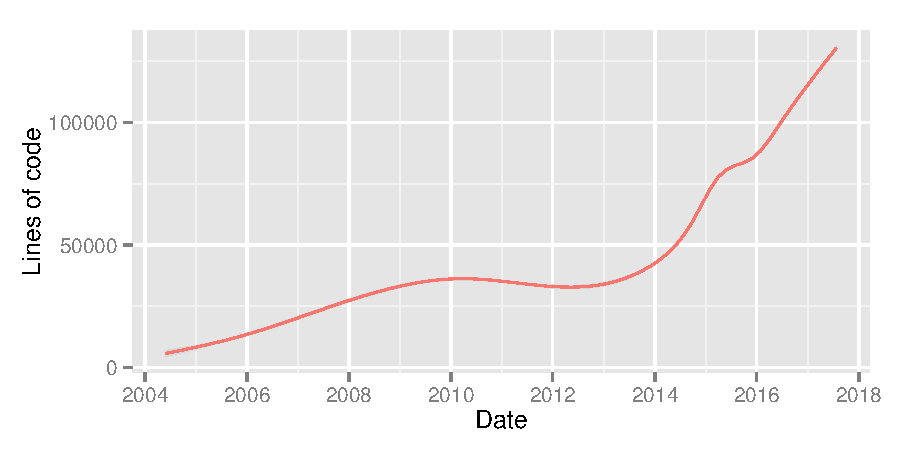
\includegraphics{history}
\caption[History of lines of code in Elektra.]{History of lines of code in Elektra as counted with Sloccount and visualized with smoothed conditional means.
}
\label{fig:elektra-history}
\end{figure}

As we see in \figref{elektra-history}, \elektra{} started in 2004 and we removed some source code around 2012.
This was mainly a cleanup of obsolete bindings (for example, python, which was reintroduced later), patches for other applications (for example, KDE and Xserver), and plugins (for example, gconf and filesys~\cite{raab2010thesis}).
Since then, the lines of code continuously grew on average.


In total, \elektra{} has 308,875 lines in all files.
Sloccount reports 128,735 lines of code, while Cloc finds 158,679 lines of code.
Sloccount gives an estimation that developing \elektra{} from scratch would cost \$4,434,280.

About 40 people participated in the development of \elektra{}, 26 of them have their names in the credits.
Using ^git blame^ we found that the author of this book is responsible for 145,534 lines.
This is the highest number from all contributors, the next person following with 41,166 lines.
The author of the book contributed 5,234 commits. %4074+699+265+170+26
In total he added 502,833 lines, and removed 574,261 lines\footnote{The small difference is caused by removing source code of others, mainly done in 2012.}.

The author reviewed at least\footnote{On GitHub alone, not counting emails and previous source code collaboration tools.} 726 patches for \elektra{}.
In the reviews we sometimes had lengthy discussions, in one review we wrote 287 comments.
In the bug tracker, \elektra{} had 223 open and 616 closed issues.
The most commented issue was about the build server with 152 comments.

The mostly used languages are
C with 63,299 lines of code,
C++ with 35,521 lines of code, and
C/C++ header with 27,488 lines of code.
The core is exclusively in C.
C++ was used for tooling and some plugins.

According to Sloccount, most of the lines of code are for tests:
about 50,877 lines of code\footnote{Estimated with Sloccount by counting folders called \texttt{tests} and files called \texttt{testmod*}.}.
The testing source code contains about 10,179 assert statements.
Non-testing source code in \elektra{Lib} has 103 assert statements and 137 logging statements.

Of the remaining 77,858 lines of non-testing code 32,429 are for the 79 plugins.\footnote{The plugin \plugin{ipaddr} was not merged at that time.}
Looking in more detail at the lines of non-testing code for the individual plugins, most plugins are fairly small:
The mean is 410 lines of non-testing code, the median is 239 lines of non-testing code.
The source code size is within the suggested optimum of 200--400 lines of code for modules~\cite{hatton1997reexamining}.
Our largest plugins are ^ni^ with 3,474 lines of non-testing code, ^crypto^ with 2,393 lines of non-testing code, and ^ini^ with 1,997 lines of non-testing code.
Our smallest plugin is ^journald^ with 53 lines of non-testing code.

\elektra{} is packaged for most GNU/Linux distributions.
Current packages (\elektra{} version 0.8) are known to exist for at least 10 distributions.
The maintainers of these distributions sometimes use distribution-specific tools that improve the quality of packages, which sometimes improves \elektra{}.
For example, on Debian's infrastructure most of \elektra{}'s unit tests run at many architectures which unveiled architecture-specific problems.
In particular, the Debian maintainer found that the source code for intercepting the function pre-^main^ (to hijack command-line arguments) needed to be different on the Powerpc architecture.

\elektra{}'s official build server has about 40 build jobs and 8 build agents.
It builds with three different compilers (GCC, Icc, Clang).
The build times are from ten minutes to half an hour if also memory leak checks are done.
We run about 8 build jobs for every patch under review and nearly all build jobs for every accepted patch.

Pmccabe reported code complexity metrics for 4,121 C/C++ functions in the 546 \elektra{}'s C/C++ source files.
The median for the code complexity is 1, and the mean is 3.7.
Two functions were extreme outliers in terms of code complexity.
They were independently developed but both in plugins related to INI parsing.
These outliers had code complexity 76 and 131.



No vulnerabilities against \elektra{} were reported.

The author of the book developed the following parts of \elektra{} by himself:
\begin{description}
\item[Core] of \elektra{Lib} contains mounting logic, lookup algorithms, and delegation of the work to plugins.
The ^KeySet^ has origins in earlier source code.
Most parts of the data structure, such as ^ksLookup^ as described in \secref{lookup}, were completely redesigned by the author.
\item[Libtools] contains algorithms assembling plugins as described in \secref{plugin-assembly}.
\item[Plugins] of the author include many small plugins (logging and encodings), some larger plugins (resolvers and validations), and some storage plugins (C, INI and JSON).
\item[\relax\elektra{Gen}] is a prototype with rudimentary error reporting.
\item[Kdb-tool] is the command-line tool suite as described in \secref{implication-command-line-interface}.
Some commands of the command-line tool suite were contributed by others.
\item[Interception] of ^getenv^ and pre-^main^ (for command-line arguments).
\end{description}



The following parts were mainly developed by students of the author:
\begin{description}
\item[Augeas] is a plugin using lenses as described in \secref{augeas}.
\item[Crypto] enables the encryption and signature of configuration files.
\item[Puppet] integrates \elektra{} into Puppet.
It supports to mount backends and to set keys using Puppet.
\item[User interfaces] of \elektra{} that include a website with snippet sharing functionality,
a graphical user interface implemented using Qt,
and a web user interface implemented using Node.js (see \secref{tooling}).
\item[3-way merge] improves merging of configuration settings as described in \secref{three-way-merge}.
\end{description}

\elektra{} has other contributors, mainly people who are users of \elektra{}.
For example, people from Oyranos (a color management framework) and Machinekit (a framework for machine control applications) have contributed to \elektra{}.


\subsection{Security Considerations}

Here we discuss if it is more secure to implement a configuration file parser (which is still a popular way, as our survey suggests) or to use \elektra{}.

From the security perspective \elektra{Lib} provides a lightweight solution.
\elektra{Lib} does not spawn new threads or processes, nor does it need any special privileges.
\elektra{Lib} is only a library that parses and serializes several configuration files.
Thus by design, \elektra{} does not make any privilege escalation possible---at least not beyond the privileges of the application.
Implementing access control checks within \elektra{} is less useful, as they are easily circumvented.
Instead isolation techniques of the file system shall be used~\cite{liang2003isolated}.

A project we started to \empha[elektrify]{elektrify} is LCDproc, a software to drive liquid-crystal displays.
Measured with Cloc, LCDproc 0.5.8 has 76,552 lines of code in total.
Configuration access code is at least 1,652 lines of code (\p{2}) which can be fully replaced by \elektra{}. % 281 from main.c
Additionally, LCDproc's modules have even more lines of code that parses configuration values.
This source code is a candidate to be replaced by source code in plugins.

We found three important security considerations:
\begin{enumerate}
\item
If a parser within \elektra{} is known to be problematic, applications can immediately switch to others, without having to wait for upstream changes.
Adding the property \property{mountpoint} to the configuration specification and reimporting configuration settings suffices.
Other configuration libraries do not have this capability.

\item
\elektra{} has more lines of code than a single configuration file parser.
For example, LCDproc's configuration file parser has 1,652 lines of code, while the core of \elektra{} has 6,103 lines of code.
From the system's perspective, however, a solution with \elektra{} can still lead to less exploitable code because \elektra{} intends to replace all other configuration file parsers, too.
Another aspect is that \elektra{Spec}'s specifications have less source code and are easier to understand than configuration validation code written in low-level languages.


\item
Instead of many mostly unmaintained and untested parsers in every application, \elektra{}'s parsers are maintained by the \elektra{} initiative.
The \elektra{} initiative uses full-automatic checkers to find security problems within the library.
We elaborate on memory safety in \elektra{} in \secref{memory-safety}.
\end{enumerate}




\subsection{Memory Safety}
\label{sec:memory-safety}

\elektra{} is mostly implemented in the programming language C, which is an unsafe programming language~\cite{matsakis2014rust}.
The \elektra{} initiative uses several techniques to mitigate the problems coming from this programming language~\cite{torri2010evaluation}:

\begin{description}
\item[Code sanitizers] make sure that \elektra{} does not have undefined behavior while executing the tests~\cite{serebryany2012addresssanitizer}.
\item[Static analysis tools] such as Cppcheck reparse the source code and yield useful additional warnings but are inherently incomplete.
\item[Valgrind] finds memory and data-race errors~\cite{nethercote2007Valgrind}.
\item[C Bounded Model Checker] (CBMC)~\cite{kroening2014cbmc} proves that assertions always hold with a source code where the loops are unrolled to a specified depth.
Because not everything is specified using assertions and because of the limitations with loops, CBMC is incomplete.
\item[American Fuzzy Lop] (AFL\footnote{A technical whitepaper on details of AFL-fuzz (American Fuzzy Lop) is found here: \url{http://lcamtuf.coredump.cx/afl/technical_details.txt}.}) is the state of the art of mutational fuzzer tools~\cite{cha2015program}. We use it to mutate configuration files and ^kdb^ scripts. While it is a highly effective solution, it is incomplete.
\item[Code complexity tools] tell us the code complexity of functions.
We use it to decide about refactoring.
\item[API design] is essential to make sure that memory-safety is not circumvented by API misuse.
Unfortunately, despite its design goals, the C API has potential to be misused because pointers are needed.
In the high-level APIs and bindings of \elektra{}, however, which are the only recommended ways to use \elektra{}, we are not aware of design flaws.%
{\parfillskip=0pt plus .8\textwidth \emergencystretch=.5\textwidth \par}
\item[Code reviews] have some chance to find anything else or at least increase the chances that the tools are not cheated.
\end{description}

Unfortunately in practice, errors slip through despite all these counter-measures.
Nevertheless, it is unlikely that applications put such efforts into their configuration access code.
So \elektra{} can increase security, despite being implemented in an unsafe language.%
{\parfillskip=0pt \emergencystretch=.5\textwidth \par}




\subsection{Misconfiguration}
\label{sec:implication-misconfiguration}

We continue with \rqref{implication-misconfiguration}:
\rqImplicationMisconfiguration*

In the introduction, we claimed that \elektra{} helps in reducing misconfigurations.
Here we discuss in which situations we expected or observed reduction of misconfigurations.
We discuss misconfigurations specific to security later in \secref{secure-configuration}.
We report on misconfigurations mentioned by \citet{xu2015systems}, \citet{nagaraja2004understanding}, and \citet{keller2008conferr}.%
{\parfillskip=0pt plus .8\textwidth \emergencystretch=.5\textwidth \par}

Whether \elektra{} is resilient against spelling mistakes in configuration files, depends on which plugins are used.
For example, different configuration file syntaxes or capitalization allowance (using the plugin \plugin{rename}) has effects on acceptance of spelling mistakes.
The largest class of spelling mistakes is covered by the extensive set of data types \elektra{} provides.
We listed all plugins implementing data types in \secref{data-types}.
Using these plugins, we were able to restrict configuration settings to exactly the allowed characters and canonicalize different allowed spellings if confusion is unlikely.
These features are beyond the features of other configuration libraries, so \elektra{} improves the situation.

For structural errors a similar reasoning is applied.
One of \elektra{}'s contributions is that different user interfaces are available.
If the tool shows the structure more clearly and gives better feedback, we increase usability.
For example, a tool suggests to change settings relevant within a hierarchy.
By design the constraints from the key set---as discussed in \chapref{approach}---cannot be violated.
The user cannot
\begin{itemize}
\item add keys into the key set with the same key name,
\item create syntactically invalid configuration files by persisting a key set, and
\item create a situation where a key is not found by the application (see \secref{approach-guarantees}).
\end{itemize}
Misconfigurations that stem from unawareness of the configuration file syntax should be greatly reduced.
Such misconfigurations should not reach applications anymore because they are already eliminated during ^kdb.set^, i.\,e., before serializing the configuration files (see \secref{kdb-api}).

With \elektra{Spec} system administrators avoid duplication of configuration settings.
They use the properties \property{override} and \property{fallback} instead.
We are positive that a reduction of duplication reduces misconfiguration because it eliminates a source of inconsistency.
Furthermore, system administrators do not need to set configuration settings that can be derived by default value calculations.

For semantic errors, the plugin system is essential.
In plugins, we check for success using the exact same APIs the application uses later.
This way we exclude whole classes of errors such as:
\begin{itemize}
\item Invalid file paths using the plugin \plugin{path}.
\item Invalid IP addresses or host names using the plugins \plugin{network} or \plugin{ipaddr}.
\end{itemize}
Because the checks occur before the resources are actually used, the checks are subject to race conditions.
For example, a path that was present during the check, can have been removed when the application tries to access it.
In some situations facilities of the operating system help,\footnote{For example, we open the file during the check and pass \texttt{/proc/<pid>/fd/<fd>} to the application. This file cannot be unlinked, but unfortunately the file descriptor requires resources.} in others we have fundamental problems.\footnote{For example, if the host we want to reach has gone offline after validation.}

Beyond misconfigurations impossible due to \elektra{}'s design, the rejection rate of misconfigurations depends on the effort put into writing \elektra{Spec} specifications.
While most of the misconfigurations described above are reliably rejected after adding a single property, sometimes more elaborate specifications are needed.
For example, \citet{nagaraja2004understanding} discussed two errors (both with ^mod_jk^):
\begin{itemize}
\item A name was added at one place, but forgotten at another place.
\item A uniqueness constraint was violated.
\end{itemize}
While such errors can be checked by configuration validations, a redesign of the key names can lead to a system where wanted constraints are always implicitly fulfilled.
For example, we designed the plugin \plugin{hosts} so that the canonical host name is part of the key name.
With such a design, violation of uniqueness is impossible due to the key set semantics.
It remains to be seen if thinking about how to write validation specifications (and trying to avoid complicated validation specifications) will lead to better design overall.

For some errors, \elektra{} needs additional information next to the specifications.
For example, \citet{nagaraja2004understanding} described a situation where the file path was valid but pointed to a slower hard disk.
To detect such situations, we would need performance requirements encoded as configuration setting and plugins that check the performance of individual folders.
It is unclear if the effort to implement such a plugin is worthwhile.
If we had such a plugin available, however, including such a check would be easy.

It is likely that \elektra{} helps in situations where users want to share configuration settings.
The presence of key names referring to configuration settings has certainly benefits compared to manually locating and manipulating configuration files.
Tutorials can use configuration settings in a format for which \elektra{} provides a reliable import.

We are positive that \elektra{} yields better error messages than most of the previous configuration libraries.
Even more important, \elektra{} provides diagnostics and trouble shooting support.
\elektra{} enables throughout introspection of all configuration settings.

We do not know yet if \elektra{} helps with compatibility problems.
Some misconfigurations are out of scope for \elektra{}.
For example, installation of applications needs to be done by configuration management tools on top of \elektra{}.

A quantitative evaluation showing significant reduction of misconfiguration, is still missing.
Nevertheless, as discussed above, \elektra{} helps in many cases of misconfigurations.

In particular, we can facilitate the main contribution of our book, i.\,e.\ context-aware configuration, to reduce misconfiguration.
We can use the configuration settings and hardware information of the system to derive configuration settings.
Ideally, the configuration settings are also automatically adapted to new situations as shown in the use case of flexible workspaces in \secref{cose-process}.




\subsection{Secure Configuration Settings}
\label{sec:secure-configuration}

Currently, in FLOSS ecosystems security patches are unable to efficiently enforce presence of specific values in configuration files.
Completely patching the insecure functionality away, however, breaks some legacy systems.
We propose to use configuration settings as requirements that specify security levels.
Once the user tries to configure the application to be too insecure, the validation checker fails.
\elektra{} guarantees that the application only receives data as specified in the configuration specification.
Distributions change the specification to enforce that insecure configuration settings are avoided.
System administrators that need to maintain legacy systems can weaken the security levels.
We do not recommend exposing the security levels to end users.

Using the introspection \elektra{} enables monitoring of security relevant configuration settings.
Tools are able to warn users about non-recommended configuration settings.
For example, \citet{nagaraja2004understanding} described a case where a study participant forgot assigning a password for the MySQL root user.
Using \elektra{}, we easily integrate checks that warn on such situations.

\elektra{} supports signing and encryption of configuration settings.
This way, unwanted tampering of configuration settings is detected.
The encryption is particularly important for configuration settings that contain passwords as often found in ^.netrc^ (a configuration file containing login data).
\elektra{} relies on security and key management of ^gpg^, which is an encryption and signing tool.

Further work is required to evaluate the security implications in more detail.

\subsection{Discussion}

We answer \rqref{implication-security} and its subquestions:
\rqImplicationSecurity*
\begin{finding}
\begin{description}
\item[Security:]
The metrics show that \elektra{} has more lines of codes than a configuration parser by itself.
Implications and risks on security are manifold:
Some risks may be higher but \elektra{} gives more ways to deal with them.

\item[Safety:]
\elektra{} avoids several classes of misconfiguration and enables us to deal with other classes, sometimes with little effort.

Due to \elektra{}'s flexibility and configurability, \elektra{} might introduce new kinds of misconfigurations.
Problems that might occur during writing the specifications were discussed in \secref{administer}.
\item[Quality:]
Users might not be aware of individual's plugins low quality.
We mitigated this issue by automatic selection of plugins.

\elektra{} makes complexity---that previously has been resolved manually by system administrators---explicit.
Potential bugs in manual configuration processes are moved to potential bugs in \elektra{}.
\end{description}
\end{finding}

